\documentclass[12pt]{article}
\usepackage{amsmath,amsfonts,amssymb}
\usepackage{graphicx}
\usepackage{physics}
\usepackage{bm}
\usepackage{geometry}
\geometry{margin=1in}

\title{Lecture 5 -- Nonlinear Response}
\date{}
\begin{document}
\maketitle

\section{Review from Last Day}
\begin{itemize}
  \item Scattering states are intuitively easy, but the exact form is often messy.
  \item No such thing as a truly localized E\&M mode in a finite system.
  \item Scattering states form a complete orthonormal basis (if we ignore material dispersion $\equiv$ loss).
\end{itemize}

\section{Non-Linear Wave Equation}
Backing up, we start with the inhomogeneous wave equation (time domain) driven by time-varying polarization $\vec{P}(\vec{r}, t)$:
\begin{equation*}
\left[ -\nabla^2 + \frac{1}{c^2} \frac{\partial^2}{\partial t^2} \right] \epsilon_0 \vec{E}(\vec{r}, t) = -\frac{\partial^2}{\partial t^2} \vec{P}(\vec{r}, t)
\end{equation*}
Let us now consider a local polarization with a non-linear (NL) component in addition to the previously examined linear (L) component:
\begin{equation*}
\vec{P}(\vec{r}, t) = \vec{P}_L(\vec{r}, t) + \vec{P}_{NL}(\vec{r}, t)
\end{equation*}
Here we are assuming a ‘local’ response which means at any given point $\vec{r}$, a polarization density $\vec{P}(\vec{r},t)$ is induced and is related to the powers of the electric field $\vec{E}(\vec{r},t)$ at that point.
\begin{equation*}
\vec{P}_L(\vec{r}, t) = \epsilon_0 \chi^{(1)}(\vec{r}) \vec{E}(\vec{r}, t) \\
\end{equation*}
\begin{equation*}
\vec{P}_{NL}(\vec{r}, t) = \epsilon_0 \chi^{(2)}(\vec{r}) \vec{E}^2(\vec{r}, t) + \epsilon_0 \chi^{(3)}(\vec{r}) \vec{E}^3(\vec{r}, t) + \dots
\end{equation*}
Even with the non-linear addition, we can still FT in $t$. By moving the linear part and $\chi^{(1)}(\vec{r})$ to the left-hand side, we have the general linear dielectric landscape on the left (which we are by now familiar with) and the driving term on the right which is specifically non-linear.
\begin{equation*}
\left[ -\nabla^2 - \tilde{\omega}^2 (1 + \chi^{(1)}(\vec{r})) \right] \epsilon_0 \tilde{\vec{E}}(\vec{r}; \omega) = \tilde{\omega}^2 \tilde{\vec{P}}_{NL}(\vec{r}; \omega)
\end{equation*}
\begin{equation*}
\left[ -\nabla^2 - \tilde{\omega}^2 \epsilon^{(1)}(\vec{r}) \right] \epsilon_0 \tilde{\vec{E}}(\vec{r}; \omega) = \tilde{\omega}^2 \tilde{\vec{P}}_{NL}(\vec{r}; \omega)
\end{equation*}
The only complication now is that by taking the FT of a product of time-dependent functions, we get a convolution in frequency space. This means we can have contributions from many frequency components of the electric field to the polarization response at a single frequency.
Nevertheless, it remains useful to find a Green’s function satisfying,
\begin{equation*}
\left[ -\nabla^2 - \tilde{\omega}^2 \epsilon^{(1)}(\vec{r}) \right] \vec{G}(\vec{r}, \vec{r'}; \omega) = \delta(\vec{r} - \vec{r'})
\end{equation*}
Then, for a given polarization $\tilde{\vec{P}}_{NL}(\vec{r}'; \omega)$ the particular solution of Maxwell's equations is determined as,
\begin{equation*}
\epsilon_0 \tilde{\vec{E}}_{\text{part}}^{TE_0}(\vec{r}; \omega) = \tilde{\omega}^2 \int \vec{G}(\vec{r}, \vec{r'}; \omega) \cdot \tilde{\vec{P}}_{NL}(\vec{r'}; \omega) d\vec{r'}
\end{equation*}
Next, we will derive an analytic expression for $\vec{G}$ in terms of scattering states that provides a nice physical interpretation of how $\tilde{\vec{P}}_{NL} (\vec{r'};\omega)$ generates new fields.

\section{Quasi-Harmonic Field Simplification}
To avoid dealing with convolutions, we will initially assume a simplification of ‘quasi-harmonic electric fields’ 
\begin{equation*}
\vec{E}(\vec{r}, t) = \vec{E}(\vec{r}; \omega_d) e^{-i\omega_d t}
\end{equation*}
Physically, this means that we are assuming the electric field oscillates at a single frequency $\omega_d$, rather than the full broadband of frequencies. 
As shown before, the general wave-equation with a non-linear polarization in the time domain is given by equation~\ref{eq:5.1}.
\begin{equation}
\left[ \nabla^2 - \epsilon^{(1)}(\vec{r}) \frac{\partial^2}{\partial t^2} \right] \epsilon_0 \vec{E}(\vec{r}, t) = \frac{\partial^2}{\partial t^2} \vec{P}_{NL}(\vec{r}, t)
\label{eq:5.1}
\end{equation}
Which takes the form of equation~\ref{eq:5.2} in the frequency domain after the FT:
\begin{equation}
\left[ -\nabla^2 - \epsilon^{(1)}(\vec{r}) \tilde{\omega}^2 \right] \tilde{\vec{E}}(\vec{r}, \omega) = \frac{\tilde{\omega}^2}{\epsilon_0} \tilde{\vec{P}}_{NL}(\vec{r}, \omega)
\label{eq:5.2}
\end{equation}
With the quasi-harmonic assumption, the FT of the electric field, and the polarization, both become much simpler (delta functions rather than convolutions):
\begin{align*}
\tilde{\vec{E}}(\vec{r}, \omega) &= \vec{E}(\vec{r}; \omega_d) \delta(\omega - \omega_d) \sqrt{2\pi} \\
\tilde{\vec{P}}(\vec{r}, \omega) &= \vec{P}_{NL}(\vec{r}; \omega_d) \delta(\omega - \omega_d) \sqrt{2\pi}
\end{align*}
Plugging in these functions for a single discrete frequency $\omega_d$ the wave equation simplifies to,
\begin{equation}
\left[ -\nabla^2 - \epsilon^{(1)}(\vec{r}) \tilde{\omega}_d^2 \right] \vec{E}(\vec{r}; \omega_d) = \frac{\tilde{\omega}_d^2}{\epsilon_0} \vec{P}_{NL}(\vec{r}; \omega_d)
\label{eq:5.3}
\end{equation}

\section{Double Bus Ring}
As $t\rightarrow-\infty$, scattering state solutions of equation~\ref{eq:5.3} will exist as the CW limit of a bound mode wave packet incoming towards the ring along one bus waveguide arm, that is necessarily a solution of the isolated straight waveguide version of equation~\ref{eq:5.3}. As $t\rightarrow+\infty$, solutions consist of a set of some outward propagating bound mode wave packets in the bus waveguides, plus some radiation outside of the waveguides.
The CW limit of these incoming scattering states will be labelled by the $k_z (\omega)$ wave vector of the incoming bound mode, and will have an un-normalized form approximately $rA_{\text{in}} e^{ik_zz} \Theta(z)$. These scattering states are visualized in figure ~\ref{fig:RingScatState}. 
\begin{figure}
    \centering
    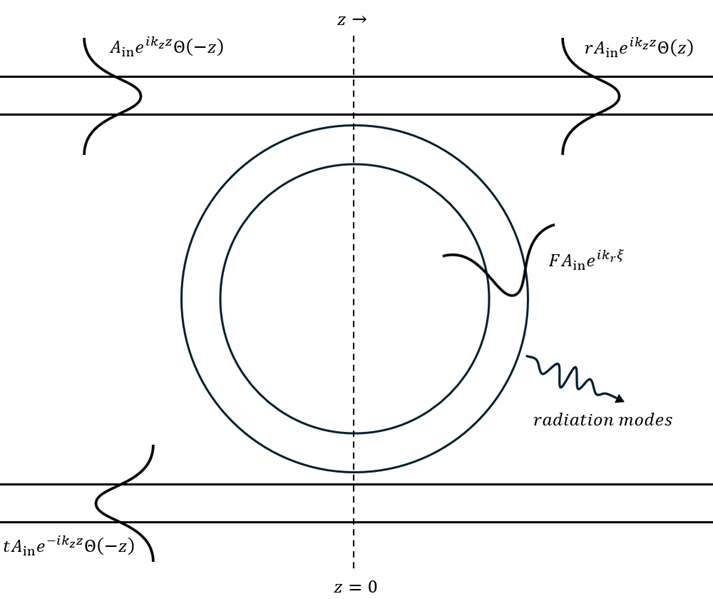
\includegraphics[width=0.7\linewidth]{Scattering_ring.png}
    \caption{Double-bus ring scattering states}
    \label{fig:RingScatState}
\end{figure}
There will also be a set of modes that are the CW limit of an outward propagating wave packet in one the waveguides as $t\rightarrow+\infty$ that was made possible by the ring being excited by a set of bound incoming waveguide modes and a set of incoming radiation modes as $t\rightarrow-\infty$.
There will also be a whole set of other scattering state solutions, both incoming and outgoing, associated with other bound transverse modes and just pure radiation modes. 
An arbitrary field distribution, $\vec{E}(\vec{r})$, can be expanded in either the complete set of incoming or outgoing scattering states.
If the exact radiation patterns of these modes are ignored, their impact on $|r|^2+|t|^2<1$ can be mimicked by adding a third ‘phantom’ waveguide channel, see figure ~\ref{fig:PhantomRing}.
\begin{figure}
    \centering
    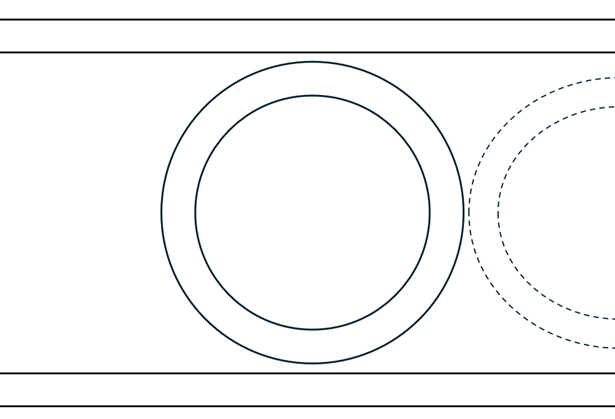
\includegraphics[width=0.7\linewidth]{Phantom_ring.png}
    \caption{Phantom channel ring}
    \label{fig:PhantomRing}
\end{figure}
If the waveguides and layout are designed properly, we can assume the subspace of one transverse bound mode’s set of incoming and outgoing scattering states, including the phantom channel, will define a closed subspace for all relevant fields in the problem. 

\section{Green's Function Calculation}
Going back to the electric field formation, at any frequency $\omega_d$, there will be a $\vec{\phi_k}^{\text{in/out}}(\vec{r})$ and a $k(\omega_d)$ satisfying,
\begin{equation*}
\left[ -\nabla^2 - \epsilon^{(1)}(\vec{r}) \tilde{\omega}_d^2 \right] \tilde{\vec{E}}_{\text{in/out}}(\vec{r}; k; \omega_d) = 0
\end{equation*}
These solutions take the form,
\begin{equation*}
\tilde{\vec{E}}_{\text{in/out}}(\vec{r}; k; \omega_d) = a_k \left( \frac{\hbar \omega_d}{2 \epsilon_0} \right)^{1/2} \frac{\vec{\phi_k}^{\text{in/out}}(\vec{r})}{\sqrt{A_k^\eta}}
\end{equation*}
The parts of this formation are the mode amplitude $a_k$, the energy normalization term $\left(\frac{\hbar\omega_d}{{2\epsilon_0}}\right)^{1/2}$, the effective mode area $\sqrt{A_k^\eta}$, and the spatial mode profile of the in-coming or out-going mode $\vec{\phi_k}^{\text{in/out}}(\vec{r})$.
\begin{equation*}
\vec{E}(\vec{r}) = \frac{1}{\sqrt{2\pi}} \int_0^\infty dk \, a_k \left( \frac{\hbar \omega_d}{2\epsilon_0} \right)^{1/2} \frac{\vec{\phi_k}^{\text{in/out}}(\vec{r})}{\sqrt{A_k^\eta}}
\end{equation*}
$\vec{E}(\vec{r})$ has units $E$, $dk$ has units $k$, $a_k$ has units $\frac{1}{\sqrt{k}}$, $\left(\frac{\hbar\omega_d}{{2\epsilon_0}}\right)^{1/2}$ has units $\frac{E}{k^{3/2}}$ , $\frac{1}{\sqrt{A_k^\eta}}$ has units $k$, and $\vec{\phi_k}^{\text{in/out}}(\vec{r})$ is unitless.
The general solution for equation~\ref{eq:5.2} is then:
\begin{equation*}
\vec{E}(\vec{r},\omega_d) = \frac{1}{\sqrt{2\pi}} \int_0^\infty dk \, a_k \left( \frac{\hbar \omega_d}{2\epsilon_0} \right)^{1/2} \frac{\vec{\phi_k}^{\text{in/out}}(\vec{r})}{\sqrt{A_k^\eta}}
\end{equation*}
Where the $a_k$ is determined by the polarization distribution $\vec{P}_{NL}(\vec{r},\omega_d )$.
Subbing $\vec{E}(\vec{r},\omega_d)$ into equation~\ref{eq:5.2} we get,
\begin{align*}
&\left[ -\nabla^2 + \epsilon^{(1)}(\vec{r}) \tilde{\omega}_d^2 \right] \frac{1}{\sqrt{2\pi}} \int dk \, a_k \left( \frac{\hbar \omega_k}{2\epsilon_0} \right)^{1/2} \frac{\vec{E}_k(\vec{r})}{\sqrt{A_k^\eta}} = \frac{\tilde{\omega}_d^2}{\epsilon_0} \vec{P}_{NL}(\vec{r}; \omega_d)
\end{align*}
Using $-\nabla^2 \vec{E}_k = \epsilon^{(1)}(\vec{r}) \tilde{\omega}_k^2 \vec{E}_k$ we get,
\begin{equation*}
\epsilon^{(1)}(\vec{r}) \frac{1}{\sqrt{2\pi}} \int dk\, (\tilde{\omega}_d^2 - \tilde{\omega}_k^2)\, a_k \left( \frac{\hbar \omega_k}{2\epsilon_0} \right)^{1/2} \vec{\phi}_k(\vec{r}) = \frac{\tilde{\omega}_d^2}{\epsilon_0} \vec{P}_{\mathrm{NL}}(\vec{r}; \omega_d)
\end{equation*}
Multiply by $\frac{\bm{\phi}^*_{k'}(\vec{r})}{\sqrt{A_{k'}^\eta}} \int d\vec{r}$,
\begin{equation*}
\frac{1}{\sqrt{2\pi}} \int dk\, (\tilde{\omega}_d^2 - \tilde{\omega}_k^2)\, a_k \int d\vec{r}\, \epsilon_0\, \epsilon^{(1)}(\vec{r})\, \vec{\phi}^*_{k'}(\vec{r}) \vec{\phi}_k(\vec{r}) \left( \frac{\hbar \omega_k}{2 \epsilon_0} \right)^{1/2} \left( \frac{1}{A_k^\eta A_{k'}^\eta} \right)^{1/2} = \tilde{\omega}_d^2 \int d\vec{r} \frac{\vec{\phi}^*_{k'}(\vec{r})}{\sqrt{A_{k'}^\eta}} \vec{P}_{\mathrm{NL}}(\vec{r}; \omega_d)
\end{equation*}
If we choose the normalization factor $A_k^\eta$ such that,
\begin{equation*}
\epsilon_0 \int d\vec{r}\, \epsilon^{(1)}(\vec{r}) \left( \frac{\hbar \omega_k}{2 \epsilon_0} \right)^{1/2} \left( \frac{\hbar \omega_{k'}}{2 \epsilon_0} \right)^{1/2} \frac{ \vec{\phi}^*_k(\vec{r}) \vec{\phi}_{k'}(\vec{r}) }{ \left( A_k^\eta A_{k'}^\eta \right)^{1/2} } = \frac{\hbar \omega_k}{2} \delta(k - k'),
\end{equation*}
then we find,
\begin{align*}
&\frac{1}{\sqrt{2\pi}} a_{k'} (\tilde{\omega}_d^2 - \tilde{\omega}_{k'}^2) \left( \frac{\epsilon_0 \hbar \omega_{k'}}{2} \right)^{1/2} = \tilde{\omega}_d^2 \int d\vec{r} \, \frac{\vec{\phi}_{k'}^*(\vec{r}) \vec{P}_{NL}(\vec{r}; \omega_d)}{\sqrt{A_{k'}^\eta}}.
\end{align*}
Solve for $a_{k'}$.
\begin{equation*}
 a_{k'} = \tilde{\omega}_d^2 \int d\vec{r} \, 2\left( \frac{\pi}{\epsilon_0 \hbar \omega_{k'}} \right)^{1/2} \frac{\vec{\phi}_{k'}^*(\vec{r}) \cdot \vec{P}_{NL}(\vec{r}; \omega_d)}{\tilde{\omega}_d^2 - \tilde{\omega}_{k'}^2} \frac{1}{\sqrt{A_{k'}^\eta}}
\end{equation*}
The particular solution is then,
\begin{equation*}
\vec{E}(\vec{r'}; \omega_d) = \tilde{\omega}_d^2 \int dk \int d\vec{r}  \frac{2}{\sqrt{2\pi}} \left(\frac{\pi}{\epsilon_0\hbar\omega_{k'}}\right)^{1/2}\left(\frac{\hbar\omega_k}{2\epsilon_0}\right)^{1/2}  \, \frac{\vec{\phi}_{k'}(\vec{r}) \vec{\phi}_{k'}^*(\vec{r'})}{\tilde{\omega}_d^2 - \tilde{\omega}_k^2} \frac{\vec{P}_{NL}(\vec{r}; \omega_d)}{A_k^\eta}
\end{equation*}
From which we extract the Green's funciton.
\begin{equation*}
G(\vec{r}, \vec{r'}; \omega_d) = \int dk \, \frac{\vec{\phi}_{k'}^*(\vec{r}) \vec{\phi}_{k'}(\vec{r})}{\tilde{\omega}_d^2 - \tilde{\omega}_{k'}^2} \frac{1}{A_{k'}^\eta}
\end{equation*}
Recall the use of the Green’s function. Given an arbitrary non-linear polarization distribution $\tilde{\vec{P}}_{NL} (\vec{r};\omega)$, we can solve for the electric field satisfying equation~\ref{eq:5.2} by performing the integration of this polarization distribution with the Green’s function shown below.
\begin{equation*}
[-\nabla^2-\tilde{\omega}^2 \epsilon^{(1)}(\vec{r})] \epsilon_0 \tilde{\vec{E}}(\vec{r};\omega)=\tilde{\omega}^2 \tilde{\vec{P}}_{NL}(\vec{r};\omega)
\end{equation*}
\begin{equation*}
\downarrow
\end{equation*}
\begin{equation*}
\epsilon_0\tilde{\vec{E}}_\text{part}(\vec{r},\omega)=\tilde{\omega}^2 \int \vec{G}(\vec{r},\vec{r'};\omega)\cdot \tilde{\vec{P}}_{NL} (\vec{r'};\omega)dr'
\end{equation*}

\end{document}
